\documentclass[10pt,landscape]{article}
\usepackage{multicol}
\usepackage{calc}
\usepackage{ifthen}
\usepackage[landscape]{geometry}
\usepackage{listings}
\usepackage{amsmath,amsthm,amsfonts,amssymb}
\usepackage{mathtools}
\usepackage{color,graphicx,overpic}
\usepackage{hyperref}
\usepackage[table, dvipsnames, xcdraw]{xcolor} % for \colorbox and named colors
\usepackage{transparent}

\usepackage{MnSymbol}
\usepackage{graphicx}
\usepackage{wrapfig}
\usepackage{tikz}

\usepackage{blindtext}

% This sets page margins to .1 inch if using letter paper, and to 1cm
% if using A4 paper. (This probably isn't strictly necessary.)
% If using another size paper, use default 1cm margins.
\ifthenelse{\lengthtest { \paperwidth = 11in}}
    { \geometry{top=0.2in,left=0.2in,right=0.2in,bottom=0.2in} }
    {\ifthenelse{ \lengthtest{ \paperwidth = 297mm}}
        {\geometry{top=1cm,left=1cm,right=1cm,bottom=1cm} }
        {\geometry{top=1cm,left=1cm,right=1cm,bottom=1cm} }
    }

% Turn off header and footer
\pagestyle{empty}

% Redefine section commands to use less space
\makeatletter
\renewcommand{\section}{\@startsection{section}{1}{0mm}%
                                {-1ex plus -.5ex minus -.2ex}%
                                {0.5ex plus .2ex}%x
                                {\normalfont\large\bfseries}}
\renewcommand{\subsection}{\@startsection{subsection}{2}{0mm}%
                                {-1ex plus -.5ex minus -.2ex}%
                                {0.5ex plus .2ex}%
                                {\normalfont\normalsize\bfseries}}
\renewcommand{\subsubsection}{\@startsection{subsubsection}{3}{0mm}%
                                {-1ex plus -.5ex minus -.2ex}%
                                {0.5ex plus .2ex}%
                                {\normalfont\footnotesize\bfseries}}
\makeatother

% Itemize to use less space
\usepackage{enumitem}
\setlist{leftmargin=*, nosep}
\setenumerate{nosep}

% Define BibTeX command
\def\BibTeX{{\rm B\kern-.05em{\sc i\kern-.025em b}\kern-.08em
    T\kern-.1667em\lower.7ex\hbox{E}\kern-.125emX}}

% Don't print section numbers
\setcounter{secnumdepth}{0}


\setlength{\parindent}{0pt}
\setlength{\parskip}{0pt plus 0.5ex}

%My Environments
\newtheorem{example}[section]{Example}

\newcommand{\Blue}[1]{\noindent{\textcolor{Blue}{\textbf{#1}}}:}
\newcommand{\Red}[1]{\noindent{\textcolor{BrickRed}{\textbf{#1}}}:}
\newcommand{\Green}[1]{\noindent{\textcolor{PineGreen}{\textbf{#1}}}:}
\newcommand{\Hint}[1]{\noindent{\textcolor{Orange}{#1}}}

\newcommand{\TODO}[1]{%
  \vspace{1em}%
  \noindent\textbf{\Large\textcolor{BrickRed}{TODO: #1}}%
  \vspace{1em}%
}

\newcommand*{\eg}{e.g.\@\xspace}
\newcommand*{\ie}{i.e.\@\xspace}
\newcommand*{\Eg}{E.g.\@\xspace}
\newcommand*{\Ie}{I.e.\@\xspace}
\newcommand*{\esp}{esp.\@\xspace}
\newcommand*{\wrt}{\ifmmode \stext{w.r.t.} \else w.r.t.\@\xspace \fi}


\usepackage{draftwatermark}
% Configure the watermark
\SetWatermarkText{Made with love by \texttt{junruren}} % Set the watermark text
\SetWatermarkScale{0.35}            % Adjust the scale of the watermark
\SetWatermarkLightness{0.9}      % Set the lightness (closer to 1 is more faded)
% -----------------------------------------------------------------------

\begin{document}
\raggedright
\scriptsize

\begin{multicols}{4}
% multicol parameters
% These lengths are set only within the two main columns
%\setlength{\columnseprule}{0.25pt}
\setlength{\premulticols}{1pt}
\setlength{\postmulticols}{1pt}
\setlength{\multicolsep}{1pt}
\setlength{\columnsep}{2pt}

\subsection{Net Present Value (NPV)}
\Blue{Discoint rate $r$} you're indifferent between receiving \$1 today and $\$\frac{1}{1+r}$ in one period.

\Blue{Present Value (PV)} \fbox{$PV(CF_t) = \frac{\colorbox{PineGreen!30}{$CF_t$}}{(1+\colorbox{Blue!30}{$r$})^{\colorbox{BrickRed!30}{$t$}}}$}
how much a cash flow (CF) at time $t$ is worth at time 0 (today). Computing a PV is often called \Hint{``discounting''}.
\textbf{Investors prefer payoffs that are \colorbox{PineGreen!30}{larger}, \colorbox{Blue!30}{safer}, and
\colorbox{BrickRed!30}{sooner}.}

\Red{NPV} \fbox{$NPV = \sum_{t=0}^{T} \frac{CF_t}{(1+r)^t}$} summs over PVs of all cash flows in a project.
\begin{itemize}
    \item \Green{Scalability} $NPV(\alpha CF_1, \dots, \alpha CF_T) = \alpha NPV(CF_1, \dots, CF_T)$
    \item \Green{Additivity} $NPV(X_1 + Y_1, \dots, X_T + Y_T) = NPV(X_1, \dots, X_T) + NPV(Y_1, \dots, Y_T)$
    \item \Green{Breaking up by time} $NPV(CF_1, \dots, CF_T) = NPV(CF_1, \dots, CF_j) + NPV(CF_{j+1}, \dots, CF_T)$
\end{itemize}

\Blue{Future Value (FV)}
\fbox{{$FV_T(CF_0) = CF_0(1+r)^T$}}
how much a cash flow at time 0 (today) is worth in $T$ periods.

\Blue{Perpetuity}
\begin{itemize}
    \item \underline{Constant} recurring cash flow $A$ forever starting \textbf{1 period from now \ie $t = 1$}: \fbox{$PV = \frac{A}{r}$}
    \item \underline{Growing} perpetuity starting \textbf{1 period from now \ie $t = 1$} with cash flow $A$, growth rate $g$: \fbox{$PV = \frac{A}{r-g} (r > g)$}
    \item \Hint{To include the cash flow at time 0, add $A$ to the PV formula above.}
\end{itemize}

\Blue{Annuity}
\begin{itemize}
    \item \underline{Constant} recurring cash flow $A$ for $T$ periods starting \textbf{1 period from now}:
        \Hint{(\Eg a loan)}
        \fbox{$PV = \frac{A}{r} \left(1 - \frac{1}{(1+r)^T}\right)$}
        \fbox{$FV = PV \cdot (1+r)^T = A \frac{(1+r)^T - 1}{r}$}
    \item \underline{Growing} annuity starting \textbf{1 period from now} with cash flow $A$, growth rate $g$ for $T$ periods.
        \begin{itemize}
            \item If $r \neq g$
                \fbox{$PV = \frac{A}{r-g} \left(1 - \frac{(1+g)^T}{(1+r)^T}\right)$};
                \fbox{$FV = A \left(\frac{(1+r)^T - (1+g)^T}{r-g}\right)$}
            \item If $r = g$
                \fbox{$PV = T \left(\frac{A}{1+r}\right)$};
                \fbox{$FV = T \cdot A \cdot (1+r)^{T-1}$}
        \end{itemize}
\end{itemize}

\Red{Annual Percentage Rate (APR) \& Effective Annual Rate (EAR)}
\fbox{$(1+EAR) = \left(1 + \frac{APR}{k}\right)^k = (1 + r)^k$}
where $k$ is the number of compounding periods per year and $r$ is the per-period (\eg monthly) interest rate.
\begin{itemize}
    \item \underline{APR} $= r \cdot k$
    \item \underline{EAR} \ie Annual Percentage Yield (APY)
\end{itemize}
\Hint{If $APR = EAR$ between two savings accounts, APR (the one with more frequent compounding) is better.}

\subsubsection{Mortgage-related terms}

\Blue{Principal} the amount of \$ \underline{borrowed} in a lending agreement.
\Eg Buy a \$1,000,000 house with a 20\% down payment, the principal is \$800,000.

\Blue{Interest}
\begin{itemize}
    \item \Green{Fixed rate} No matter what happens to interest rates around the world, you would still be charged
        interest at this same rate.
    \item \Green{Adjustable rate (ARM)} \Eg an adjustable rate of 3\% \underline{above} the federal funds rate (the
        Fed's benchmark rate). If this rate is around 4.5\%, you would be charged a 7.5\% interest rate. If in the next
        month the Fed raises to 5\%, you would be charged an 8\% interest rate.
\end{itemize}

\Blue{Amortization schedule} sequence of payments made through the loan's lifetime. A part of the payments goes to
reduce (\ie amortize) the principal owed, and the rest goes to pay the interest on the loan.

\Blue{Collateral} An asset offered by the borrower as a guarantee in a loan. If you fail to make payments, the bank can
take the collateral.

\Blue{Refinancing} Paying off an existing loan with a new loan that has better terms. \Eg lower interest rate, lower
monthly payment, shorter loan term.

\Green{\Eg} a 30-year fixed-rate mortgage, APR 9\% compounded monthly. Fixed monthly payment $= \$3000$. First payment
will start next month and last until the contract expires in 30 years.
\begin{itemize}
    \item \Green{How much borrowed when took out the mortgage?}
        use the constant annuity formula, where
        \Hint{$A = \mathdollar 3000$, $r = \frac{0.09}{12} = 0.0075$, $T = 30 \times 12 = 360$}.
        $PV = \frac{A}{r} \left(1 - \frac{1}{(1+r)^T}\right) = \frac{3000}{0.0075} \left(1 - \frac{1}{(1+0.0075)^{360}}\right) = \mathdollar 372,845.60$
    \item \Green{10 years later, how much must pay back to the bank if sell the house?}
        (\ie NPV of the remaining principal amount as of this future date.)
        \Hint{$T = 20 \times 12 = 240$}
        $PV = \frac{3000}{0.0075} \left(1 - \frac{1}{(1+0.0075)^{240}}\right) = \mathdollar 333,434.86$
    \item \Green{Why the remaining principal is still so high after 10 years' worth of repayments?}
        \Hint{Because the amortization schedule is front-loaded.} \Ie Early on in the life of the mortgage, the vast majority
        of each monthly payment is interest: interest is applied to the remaining principal amount, and this remaining
        principal is highest in month 1 and decreases over time. Because the majority of each monthly payment in the
        early years is interest, the principal repayment amounts are small, and the remaining principal de-creases very
        slowly. (It's only toward the end of the mortgage that interest payments decline enough to repay the principal
        more quickly.)
\end{itemize}

\Red{Inflation $i$} the change in CPI \fbox{$1 + i_{t+1} = \frac{CPI_{t+1}}{CPI_t}$}
\begin{itemize}
    \item \Green{``Nominal''} \underline{not} adjusted for inflation
    \item \Green{``Real''} adjusted for inflation
\end{itemize}

\Blue{Real rate of return}
\fbox{$r_{\text{real}} = \left(\frac{1 + r_{\text{nominal}}}{1 + i} - 1\right) \approx \left(r_{\text{nominal}} - i\right)$}
\Hint{If $i$ is too high, don't use the approximation (too off).}

\Blue{Treat inflation consistently for NPV}

\fbox{$PV(CF_T) = \frac{CF_{\text{nominal,T}}}{(1 + r_{\text{nominal,T}})^T} = \frac{CF_{\text{real,T}}}{(1+r_{\text{real,T}})^T}$}
(``$_{,T}$'' denotes the cash flow at time $T$)

\Green{\Eg \underline{False} statement}
\textit{If inflation is zero, two projects paying \$100 in different years have the same NPV.}
\Hint{Time value of money still applies; later payments are worth less.}

\subsection{Capital Budgeting}

To maximize value, take on \Hint{only projects with positive NPV}.
\begin{itemize}
    \item \Green{Single} take it only if it has positive NPV.
    \item \Green{Independent} take all with positive NPV.
    \item \Green{Mutually exclusive} take the one with the highest positive NPV.
    \item \Hint{Ignore} sunk costs, including opportunity costs.
\end{itemize}

\Red{\underline{Cash} operating expenses}
\begin{itemize}
    \item \Blue{COGS} direct costs attributable to the production of the goods sold by a business.
    \item \Blue{R\&D} costs associated with discovering new knowledge or develop new products, processes, and services.
    \item \Blue{SG\&A} costs not directly tied to the production of goods. \eg ``S'': advertising and sales commissions. ``G'': salaries of non-production personnel. ``A'': legal, accounting, and exec salaries.
\end{itemize}

\Blue{Depreciation} \underline{non-cash} expense that reduces the value of an asset over time. \Hint{For most finance
problems, we want to strip out effects of depreciation to get back to free cash flow.} Exception: if depreciation
affects free cash flows through taxes.

\Red{EBITDA} \fbox{$= (\text{Op. Rev.}) - (\text{All Op. Exp. w/o depreciation})$}

\Red{EBIT} \fbox{$= \text{EBITDA} - \text{Depreciation (\& Amort.)}$}

\Red{Cash Flows} from accounting statements
\fbox{$CF = (1 - \tau) (\text{EBITDA}) + \tau (\text{Dep.}) - (\text{CapEx}) - \Delta \text{WC}$}
\fbox{$CF = (1 - \tau) (\text{EBIT}) + (\text{Dep.}) - (\text{CapEx}) - \Delta \text{WC}$}

\Red{Working Capital (WC)} \fbox{$= \text{Inventory} + \text{A/R} - \text{A/P}$}
We are about \Hint{changes (\ie $\Delta$) in WC, not levels} because if keeping WC constant, no new cash flow required.

\subsubsection{Valuing Firms (usual approach)}

\begin{itemize}
    \item Forecasted $CF_1$ through $CF_N$
    \item Assume constant growth at rate $g$ after year $N$.
\end{itemize}

Then enterprise value as of today ($t = 0$):
\fbox{$EV = \colorbox{blue!30}{$\left(\sum_{t=1}^{N} \frac{CF_t}{(1+r)^t}\right)$} + \colorbox{purple!30}{$\frac{\textcolor{PineGreen}{TV_N}}{(1+r)^N}$}$}

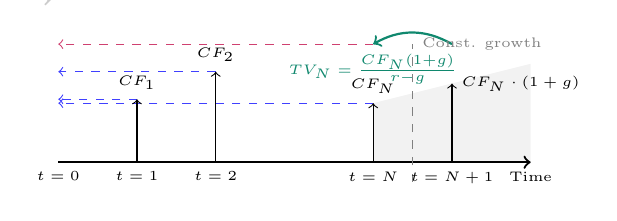
\begin{tikzpicture}
    % Loss
    \fill[gray!10] (4, 0) -- (4, 0.75) -- (6, 1.25) -- (6, 0) -- cycle;
    \draw[->,blue!75,dashed] (1,0.8) -- (0,0.8);
    \draw[->,blue!75,dashed] (2,1.15) -- (0,1.15);
    \draw[->,blue!75,dashed] (4,0.75) -- (0,0.75);
    \draw[->,purple!75,dashed] (4,1.5) -- (0,1.5);
    % Draw lines
    \draw[->,thick] (0,0) -- (6,0) node[anchor=north] {\tiny Time}; % Time axis

    \draw[->] (1,0) -- (1,0.8) node[anchor=south] {\tiny $CF_1$};
    \draw[->] (2,0) -- (2,1.15) node[anchor=south] {\tiny $CF_2$};
    \draw[->] (4,0) -- (4,0.75) node[anchor=south] {\tiny $CF_N$};
    \draw[->] (5,0) -- (5,1) node[anchor=west] {\tiny $CF_N \cdot (1+g)$};

    \draw[->,PineGreen,thick] (5,1.5) to [out=150, in=30] (4,1.5) node[anchor=north] {\tiny $TV_N = \frac{CF_N(1+g)}{r-g}$};
    

    \draw[dashed,gray] (4.5, -0.25) -- (4.5, 1.5) node[anchor=west] {\tiny Const. growth};
    
    % Label values
    \node[anchor=north] at (0,0) {\tiny $t = 0$};
    \node[anchor=north] at (1,0) {\tiny $t = 1$};
    \node[anchor=north] at (2,0) {\tiny $t = 2$};
    \node[anchor=north] at (4,0) {\tiny $t = N$};
    \node[anchor=north] at (5,0) {\tiny $t = N + 1$};

\end{tikzpicture}

\Green{Hotspur example}
$N = 12$ (2019) \ie year 13 begins the constant growth.
\includegraphics[width=\columnwidth]{CF.png}
\includegraphics[width=\columnwidth]{Terminal.png}
\includegraphics[width=\columnwidth]{DCF.png}
Also \Hint{CF in year 0 is not added to the EV.}
\Red{Enterprise Value (EV)} PV of future CFs
$EV = \sum_{t=1}^{\infty} PV(CF_t)$
\ie estimated via discounted CF (DCF) analysis.

\Blue{From EV to Equity Value}
$\colorbox{orange!25}{\text{MV of Equity}}
= \colorbox{blue!25}{\text{Value of operations (EV) + Non-operational assets}}
- \colorbox{red!25}{\text{MV of Debt}}$

For Hotspur, $\colorbox{blue!25}{Value of Assets} = EV + \text{(Cash \& equivalents)} + \text{(Investments available for sale)}$
$\colorbox{red!25}{\text{MV of Debt}} = \text{(Long-term debt)}$

\subsubsection{Alternatives to NPV}

\Red{Internal rate of return} discount rate that makes zero NPV.
\fbox{$NPV = \sum_{t=0}^{T} \frac{CF_t}{(1+IRR)^t} = 0$}
Determine some fixed $IRR^*$ \ie ``threshold rate'':
\begin{itemize}
    \item \Green{Independent} take if $IRR > IRR^*$.
    \item \Green{Mutually exclusive} take the one with the highest $IRR$ among projects $IRR > IRR^*$.
\end{itemize}
IRR leads to the same decision as NPV if:
\begin{itemize}
    \item Cash outflow occurs only at time 0
    \item Only one project is being considered
    \item Opportunity cost of capital (discount rate $r$) remains constant for all periods
    \item $IRR^* = r$
\end{itemize}

\Hint{Shortcomings}: no solution, multiple solutions, project size not accounted for, different projects' horizons
not fully considered.

\Green{\Eg \underline{False} statement}
\textit{If project A's NPV is larger than project B's, then the IRR of investing in project A is always higher than that
of project B.}
\Hint{The IRR could yield incongruent predictions in capital budgeting compared to the NPV rule.}

\Green{\Eg \underline{False} statement}
\textit{XZ Company is considering purchasing a copper mine, which requires an initial investment in the first year,
followed by positive cash flows for 30 years, but a large closure cost in year 31. IRR is a good method for analyzing
this investment.}
\Hint{Not a good metric when there are negative CFs after time 0, as it may yield multiple IRRs}

\Red{Payback period} min. length of time $k$ such that sum of CFs from a project is positive.
\fbox{$\sum_{t=1}^{k} CF_t \ge - CF_0 = I_0$} Determine some fixed threshold $k^*$:
\begin{itemize}
    \item \Green{Independent} take if $k \le k^*$.
    \item \Green{Mutually exclusive} take the one with the minnimum $k$ among projects $k \le k^*$.
\end{itemize}

\Red{Discounted payback period} ditto but discount CFs.
\fbox{$\sum_{t=1}^{k} \frac{CF_t}{(1+IRR)^t} \ge - CF_0 = I_0$}

\Hint{Shortcomings}: ignores CFs after $k$ and project size.

\Red{Profitability index (PI)} ratio of the NPV of future CFs to the initial investment.
\fbox{$PI = \frac{NPV}{I_0}$}
\begin{itemize}
    \item \Green{Independent} take all $PI > 1$.
    \item \Green{Mutually exclusive} take the one with the highest $PI$ and $PI > 1$.
\end{itemize}

\Hint{Shortcomings}: doesn't account for project size.

\subsection{Bonds}

\Red{Face value \ie ``par value'' / ``principal''} the value of a bond that appears on its face and that will be paid to the investor by the issuer at
maturity.

\Red{Coupon} interest paid on a bond's face value on a periodic basis prior to maturity.

\Red{Spot interest rate $r_t$} the market interest rate for discounting a signle risk-free cash flow
\underline{at horizon $t$}.

\Blue{Zero coupon bond} a bond that pays no coupons and is sold at a discount to its face value.
Price of a \$1 ZC bond with maturity $T$ is \fbox{$P_T = \frac{\mathdollar 1}{(1+r_T)^T}$}.
\Hint{We can infer spot interest rates from different ZC bond prices.}
\fbox{Given $P_T \Rightarrow r_T = \left(\frac{\mathdollar 1}{P_T}\right)^{\frac{1}{T}} - 1$}.

\Blue{Coupon bonds} with periodic coupon payments of $C_t$ and face value $F$.
Price of a coupon bond is
\fbox{$P = \left(\sum_{t=1}^{T} \frac{C_t}{(1+r_t)^t}\right) + \frac{F}{(1+r_T)^T} = \left(\sum_{t=1}^{T} C_t \cdot P_t^{\text{ZC}}\right) + F \cdot P_T^{\text{ZC}}$}.

\Red{Yield to maturity (YTM)} the discount rate $y$ that makes the PV of a bond's future cash flows equal to its price.
\fbox{$P = \left(\sum_{t=1}^{T} \frac{C_t}{(1+y)^t}\right) + \frac{F}{(1+y)^T}$} For ZC bonds, the YTM is equal to the spot interest rate \fbox{$y = r_T$}.

\Green{\Eg Bond Arbitrage} construct a trading strategy based on a mixture of bonds to generate an arbitrage profit.
\begin{enumerate}[label=\Alph*.]
    \item 1-year ZC bond: FV: \$1, price \$0.8
    \item 2-year ZC bond: FV: \$105, price \$100
    \item 2-year 5\% bond: FV: \$100, price \$106
\end{enumerate}
\begin{enumerate}
    \item Infer spot rates from ZCBs:
        \begin{tabular}{cc}
            \hline
            Maturity & Spot Rate \\
            \hline
            1 & $\frac{1}{0.8} - 1 = 0.25$ \\
            2 & $\left(\frac{105}{100}\right)^{\frac{1}{2}} - 1 \approx 0.0247$ \\
            \hline
        \end{tabular}
    \item Calculate the no-arbitrage price of the coupon bond using spot rates:
        $P = \frac{5}{(1+0.25)} + \frac{105}{(1+0.0247)^2} \approx 103.999$
        which is less than the market price of \$106.
    \item \Hint{Intuition: The coupon bond is \underline{overpriced}, so sell it and buy the ZC bonds.}
    \item Goal: Use ZC bonds to replicate the coupon bond's \underline{future} cash flows.
        \begin{tabular}{c|ccc}
            \hline
            Assume Buying & Bond & $CF_1$ & $CF_2$ \\
            \hline
            $x$ & 1-year ZC & 1 & 0 \\
            $y$ & 2-year ZC & 0 & 105 \\
            \hline
            1 & 5\% bond & 5 & 105 \\
            \hline
        \end{tabular}
    \item Solve for $x$ and $y$:
        $\begin{cases}
            1 x + 0 y &= 5 \\
            0 x + 105 y &= 105
        \end{cases} \Rightarrow \begin{cases}
            x = 5 \\
            y = 1
        \end{cases}$
    \item At $t = 0$, buy 5 1-year ZC bonds and 1 2-year ZC bond (costs $5 \times \mathdollar 0.8 + 1 \times \mathdollar 100 = 104$)
        and sell 1 coupon bond (earning \$106). This generates \$2 arbitrage profit.
\end{enumerate}

\Red{Expectations hypothesis (EH)} the yield curve reflects the market's expectations of future interest rates.
\Ie Long-term interest rates are equal to the \underline{geometric average} of short-term interest rates until maturity.
\Hint{Intuition: investors indifferent between long bond and rolling over short bond.}
\Green{\Eg 2-year rate should be given by}
\fbox{$(1 + \textcolor{violet}{r_{t,2}})^2 = (1 + \textcolor{purple}{r_{t,1}})\left(1 + \textcolor{NavyBlue}{E_t(r_{t+1,1})}\right)$},
where \begin{itemize}
    \item \textcolor{purple}{$r_{t,1}$: the 1-year rate at time $t$ (\eg today)}
    \item \textcolor{violet}{$r_{t,2}$: the 2-year rate at time $t$ (\eg today)}
    \item \textcolor{NavyBlue}{$E_t(r_{t+1,1})$: expectation at time $t$ (\eg today) of the 1-year rate that will exist at time $t+1$}
\end{itemize}

\Blue{More generally} yields reflect a component related to expectations about future short-term interest rates plus an
additional term reflecting a risk premium reflecting the uncertainty about fluctuations in future interest rates:
\fbox{$(1 + r_{t,2})^2 = (1 + r_{t,1})\left(1 + E_t(r_{t+1,1})\right) + \text{Risk Premium}$},

\Green{\Eg bond risks} interest rate changes, inflation, credit/default

\subsubsection{Duration}

\Red{(Macaulay) Duration} the weighted average time to receive the bond's cash flows.
Tells how long you have to wait to receive the average dollar from owning that bond in PV-weighted terms.
\fbox{$D = \frac{1}{P} \sum_{t=1}^{T} t \cdot PV(CF_t) = \frac{1}{P} \sum_{t=1}^{T} t \cdot \frac{CF_t}{(1+y)^t}$}
\Hint{Zero-coupon bonds' duration is equal to their maturity.}
All else equal, \Hint{coupon bond has shorter duration than zero-coupon bond; higher coupon means lower duration}.

\Red{Modified duration}
\fbox{$MD = \frac{D}{(1+y)}$} the sensitivity of a bond's price to changes in interest rates.

\Blue{Price change estimate} accurate for small changes in $y$ \fbox{$\frac{\Delta P}{P} \approx -MD \times \Delta y$}
which shows that \Hint{duration measures bond exposure to interest-rate risk}.
The higher the (modified) duration of a bond, the more its price moves ($\Delta P$) given a small change in interest
rates ($\Delta y$).
\Hint{Longer duration $\Rightarrow$ more sensitive to interest rate changes.}

\Red{Duration matching (\ie immunization)} matching the duration of assets and liabilities to eliminate interest rate risk.
\fbox{$\frac{D^{\text{Assets}}\cdot \Delta y}{1 + y} P^{\text{Assets}} \approx \frac{D^{\text{Liab.}}\cdot \Delta y}{1 + y} P^{\text{Liab.}}$}
If the value of assets ($P^A$) equal to value of liabilities ($P^L$) (usually the case), then \Hint{matching durations of two immunizes
portfolio from interest-rate risk}.
\begin{itemize}
    \item \fbox{If $P^A \neq P^L$, we need to set $D^A P^A = D^L P^L$} to immunize.
    \item Value of portfolio unchanged for small movements in $y \Rightarrow$ hedged against interest-rate risk.
    \item $D^A > D^L$ bets rates will stay constant or decrease
    \item $D^A < D^L$ bets rates will increase.
    \item This is only a \Hint{local} approximation. If interest rates change, need to \Hint{rebalance} the portfolio.
\end{itemize}

\Green{\Eg \underline{False} statement}
\textit{You're uncertain about future interest rates, but your expectation is that they will stay unchanged relative to
today. It's therefore risk-free to issue short-term bonds and invest the proceeds in long-term bonds with higher yields,
and no bank that follows this strategy will ever go bankrupt.}
\Hint{\textbf{Think SVB.} If the duration of assets exceeds the duration of liabilities, then the bank is exposed to
interest-rate risk. If interest rates increase, then the value of assets will decrease more than the value of
liabilities, and the bank may not be able to repay its short-term debt.}

\Red{Default risk} a debt issuer fails to make interest or principal payments when due.
Consider a ZCB. Let $q$ be the probability of the bond pays the promised payoff (\ie $(1-q)$ it defaults), the price of
this bond:
\fbox{$P = \frac{q \times \mathdollar 1 + (1-q) \times 0}{1 + r}$}.
\Blue{Ratings} assess the probability of default of bonds, by agencies like Moody's, S\&P, Fitch.

\subsection{Stocks}

\Red{Common stocks} equity or ownership shares in a corporation. Give right to payments; uncertain in timing and magnitude.
\begin{itemize}
    \item \Blue{Dividends} periodic payments to shareholders.
    \item \Blue{Residual claim} to assets and cash flows after all other creditors (\eg debtholders) have been paid.
    \item \Blue{Voting rights} elect board of directors, approve major corporate actions.
    \item \Blue{Limited liability} shareholders not personally liable for company's debts.
\end{itemize}

\Red{Primary market} where firms issue securities.
\begin{itemize}
    \item \Blue{Underwriting} in an IPO, investment bank buys securities from issuer and resells to public while taking the underwriting spread as profits.
    \item \Blue{Venture capital} is raised from investment partnerships, investment institutions, or wealthy individuals.
    \item \Blue{Secondary (seasoned) offering} when a public company issues additional shares to the public.
\end{itemize}

\Red{Secondary market} where investors trade previously issued securities.
\begin{itemize}
    \item \Blue{Exchanges} \eg NYSE, NASDAQ
    \item \Blue{Over-the-counter (OTC)} markets
\end{itemize}

\subsubsection{Stock Valuation}

\Red{Discounted Dividend Model (DDM)} price equals discounted future dividends.
\fbox{$P_0 = \sum_{t=1}^{\infty} \frac{D_t}{(1+r_t)^t}$}

\Red{Gordon growth model} a special case of DDM where dividends grow at a constant rate $g$.
\fbox{$P_0 = \frac{D_0 \cdot (1+g)}{r-g} = \frac{D_1}{r-g} = \textcolor{orange}{\frac{ROE - g}{r-g} \cdot BV_0}$}
Current stock price depends on the firm's BV, ROE, growth rate, and discount rate.
\begin{itemize}
    \item \Hint{If $ROE = r$}, then the price of the stock is exactly equal to the book value of equity.
    \item \Hint{If $ROE > r$}, reinvesting more increases shareholder value. \Hint{Optimal to reinvest} \ie investment
        opportunities that earn expected returns higher than the cost of capital. More common early in the life cycle of
        the firm.
    \item \Hint{If $ROE < r$}, reinvesting more destroys shareholder value. \Hint{Optimal not to reinvest} \ie return
        excess cash to shareholders. More common later in the life cycle of the firm where higher growth can be costly.
\end{itemize}

\Hint{If stock's growth pattern is forecasted to change over time, typically compute early-stage PV explicitly and then terminal value.}

\Red{Forcasting dividends $D_t$} firm investment determines dividend growth. Always a trade-off between (1) growning the
firm and (2) paying out dividends.
\begin{itemize}
    \item \Blue{Earnings Per Share (EPS)} net profit after taxes \fbox{$EPS = BV \times ROE$}
    \item \Blue{Dividend Payout Ratio} \fbox{$p = \frac{\text{Dividends}}{\text{Net Income}} = 1 - b$}
    \item \Blue{Retained earnings} \fbox{$\text{Net Income} - \text{Dividends}$}
    \item \Blue{Plowback Ratio} \fbox{$b = \frac{\text{Retained Earnings}}{\text{Net Income}}$}
    \item \Blue{Book value of Equity} cumulative retained earnings \fbox{$\text{BV} = \text{Assets} - \text{Liabilities}$}
    \item \Blue{Return on Equity (ROE)} how efficiently firm uses equity to generate profits \fbox{$\frac{\text{Net Income}}{\text{BV}}$}
    \item \Blue{Dividend growth rate} BV grows from R.E. If $ROE$ and $b$ are constant, $g$ is constant.
        \fbox{$g = b \cdot ROE = \frac{\Delta BV}{BV} = \frac{\text{Retained Earnings}}{\text{Net Income}} \times \frac{\text{Net Income}}{BV}$}.
    \item \Blue{Change in book value} \fbox{$\Delta \text{BV} = b \cdot ROE \cdot  \text{BV}$}
\end{itemize}
\begin{align*}
        \text{Dividends} &= \text{Net Income} - \text{Retained Earnings} \\
        &= BV \cdot ROE - \Delta BV \\
        &= BV \cdot ROE - b \cdot ROE \cdot BV \\
        &= (1-b) \cdot ROE \cdot BV \\
        &= p \cdot ROE \cdot BV
\end{align*}
\includegraphics[width=1\columnwidth]{organic_growth.png}

\Green{\Eg What should be Firm ABC's stock price today} (last day of year 0)
\begin{itemize}
    \item Book value of \$37.80 (per share) at the end of year 0.
    \item Growth plan is to reinvest 80\% of its earnings next year.
    \item After that, it will focus on returning cash to shareholder beginning in year 2, paying out 60\% of its
        earnings as dividends.
    \item From year 3 onwards, ABC will pay out 80\% of earnings and plans to maintain this payout policy forever.
    \item Assume that the market is expecting an ROE of 10\% for years 1 and 2, and an ROE of 8\% from year 3 onwards,
    \item Assume a constant discount rate of 8\%.
\end{itemize}

\newcommand{\calc}[1]{\textcolor{red}{#1}}
\begin{tabular}{r|cccc}
    & 0 & 1 & 2 & 3 \\
    \hline
    ROE & \cellcolor[HTML]{EFEFEF} & 10\% & 10\% & 8\% \\
    EPS & \cellcolor[HTML]{EFEFEF} & \calc{\$3.78} & \calc{\$4.08} & \calc{\$3.40} \\
    Begin BV & \cellcolor[HTML]{EFEFEF} & \calc{\$37.80} & \calc{\$40.28} & \calc{\$42.46} \\
    Payout $p$ & \cellcolor[HTML]{EFEFEF} & \calc{20\%} & 60\% & 60\% \\
    Plowback $b$ & \cellcolor[HTML]{EFEFEF} & 80\% & \calc{40\%} & \calc{40\%} \\
    End BV & \$37.80 \tikz[baseline, overlay]{\draw[->, thick, purple] (0,0.1) to node[above, font=\scriptsize] {} (0.5,0.8);} & \calc{\$40.82} \tikz[baseline, overlay]{\draw[->, thick, purple] (0,0.1) to node[above, font=\scriptsize] {} (0.5,0.8);} & \calc{\$42.46} \tikz[baseline, overlay]{\draw[->, thick, purple] (0,0.1) to node[above, font=\scriptsize] {} (0.5,0.8);} & \calc{\$43.14} \\
    Div./share & \cellcolor[HTML]{EFEFEF} & \calc{\$0.76} & \calc{\$2.45} & \calc{\$2.72} \\
    Term. Val. & \cellcolor[HTML]{EFEFEF} &  & \calc{\$42.46} &  \\
    $\sum$ CFs & \cellcolor[HTML]{EFEFEF} & \calc{\$0.76} & \calc{\$44.91} &  \\
    Discnt Fac & \cellcolor[HTML]{EFEFEF} & \calc{1.08} & \calc{1.17} &  \\
    $PV(CFs)$ & \cellcolor[HTML]{EFEFEF} & \calc{\$0.70} & \calc{\$38.50} &  \\
    Stock Price &  & \cellcolor[HTML]{EFEFEF} & \cellcolor[HTML]{EFEFEF} & \cellcolor[HTML]{EFEFEF} \\
\end{tabular}

\subsection{Capital Structure}
Structure of investors' claims to the firm's assets and future cashflows.

\Red{Modigliani-Miller Theorem} Capital structure is irrelevant to the firm's value. The
theorem requires strong assumptions:
\begin{itemize}
    \item No taxes
    \item No transaction costs or bankruptcy (or financial distress) costs
    \item Markets are efficient (rational investors, no information asymmetries)
    \item Markets are complete (for any risk, can buy/sell a contract on it)
    \item Investment decisions are fixed (regardless of choice of financing)
\end{itemize}
Under M\&M
\begin{itemize}
    \item \Blue{Market value of the firm} is unaffected by cap struct, so \fbox{$E = A - D$}
    \item \Blue{Discount rate of the firm (\ie ``risk of the firm's assets'')} weighted average of the discount rates of debt and equity:
    \fbox{$r_A = r_D \frac{D}{D + E} + r_E \frac{E}{D + E}$} where \begin{itemize}
        \item \Green{$D$} market value of debt (\$); \Green{$E = A - D$} MV of equity (\$)
        \item \Green{$r_D$} cost of debt
        \item \Green{$r_E$} cost of equity
    \end{itemize}
    \item \Blue{M\&M Proposition 2} \Hint{Higher the leverage, risker equity becomes.}
    $r_E = r_A + \frac{D}{A-D}(r_A - r_D)$
\end{itemize}

\Red{Weighted Average Cost of Capital (WACC)} weighted avg of the costs of debt and equity \Hint{after taking into account the tax shield benefit of debt}:
\fbox{$r_{\text{WACC}} = (1- \tau) r_D \frac{D}{D+E} + r_E \frac{E}{D+E}$} where $\tau$ is marginal corporate tax rate.

\Blue{Valuation using WACC}
\fbox{$V_0 = \sum_{t=1}^{\infty} \frac{CF_t}{(1 + r_{\text{WACC}})^t}$}
where \Green{$CF_t$} cashflows using standard formula assuming no tax shield benefit od debt.

\Red{Leverage costs} more leverage has costs becayse of the potential for financial distress and/or bankruptcy, which increase the cost of borrowing.

\Red{Optimal capital structure} in theory, when WACC is minimized and firm value is maximized.
\begin{itemize}
    \item Initially, the value of the firm increases in leverage, as interest pymts are tax deductible and there's little likelihood of experiencing financial distress costs.
    \item As leverage increases, the risk of the firm increases and distress costs becomes large.
    \item At the firm's optimal lverage ratio, the gain from tax shield is just offset by the cost of distress, \Hint{maximizing the value of the levered firm $V_L$}.
\end{itemize}
\includegraphics[width=0.95\columnwidth]{Optimal_Capital_Structure.png}

\subsection{Financing a Startup}

\Red{Venture Capital (VC)} provides funds to build companies from the earliest stages to freestanding, mature orgs; provides managerial advice.

\Blue{Limited Partners (LPs)} institutional/high net-worth investors providing \textit{capital} to VC funds, not involving in the fund management.

\Blue{General Partners (GPs)} pick and manage the investments within the fund, earn fees and percentage of profits. Liable for the fund's actions.

\Red{Term sheet} outline of terms and conditions in VC investment. Common features:
\begin{itemize}
    \item \Blue{Staged commitment of captal} capital provided in multiple rounds.
    \item \Blue{Pre-money/post-money valuation} before/after a round of funding. \Ie \fbox{Post-money val = Pre-money val + Paid-in capital}
    \item \Blue{Convertible security} resembles a debt instrument that can be converted into common stock at a pre-specified rate.
    \item \Blue{Convenants} contract provisions to establish governance of firms. \begin{itemize}
        \item Financial: failure to meet financial targets can affect conversion ratio of stock and preferred voting rights.
        \item Negative: restriction on indebtedness or new securities issuance; purchase of assets is subject to investor approval.
        \item Affirmative: property rights provisions and patents; disclosure rights, etc.
    \end{itemize}
    \item \Blue{Registration rights} define exit options for VC and entrepreneur. \begin{itemize}
        \item Redemption: investors can sell stock back to firm at par price plus dividend.
        \item Piggy-back registration: investors can register their unregistered stock when either the company or another investor initiates a registration (\eg, during IPO process). Allows investors (including founders and VCs) to sell a large stake at IPO.
    \end{itemize}
    \item \Blue{Preferred stock shares} have \textit{liquidation preference} over common stock shares and have a FV with \textit{redemption rights}.
\end{itemize}

\subsubsection{Relative valuation}

\Red{Equity multiples} scale the value of equity by a measure of earnings after interest pymts are made. \Eg P/E ratio $= \frac{\text{Stock price}}{EPS}$

\Red{Forward-looking P/E multiples}
\fbox{$\frac{P_0}{EPS_1} = \frac{p}{r-g}$} implied by Gordon growth model where $p$ is plowback ratio.

\subsection{Diversification}

\subsubsection{Asset return characteristics}

Buy an asset (\eg a stock) at $t = 0$ at price $P_0$. At time $t = 1$,
\begin{itemize}
    \item its cash flow (dividend) is $D_1$, and
    \item its price is $P_1$
\end{itemize}
(both are random variables). The risk-free rate is $r_F$.

\Blue{Realized return}
\fbox{$r_1 = \frac{D_1 + P_1}{P_0} - 1$}
Returns comes from both dividends and capital gains.

\Blue{Expected return}
\fbox{$E[r_1] = \frac{E[D_1] + E[P_1]}{P_0} - 1$}

\Blue{Excess return} (realized)
\fbox{$r_1 - r_F$}

\Blue{Risk premium} (expected excess return) \fbox{$E[r_1] - r_F$}

\Red{Mean (average) return}
\fbox{$\bar{r} = E[r] = \frac{1}{T} \sum_{t=1}^T r_t$}
Would be same as the expected return $E[r_t]$ if expected returns are constant for all $t$.

\Blue{Estimate Expected Return}
\begin{itemize}
    \item if have multiple possible scenarios for returns and know the probability of each scenario, use:
    \fbox{$E[r] = \sum_{i=1}^N p_i r_i$}
    \item if have a time series of past $T$ observations of returns, estimate sample estimate of expected return $\bar{r}$ as:
    \fbox{$\hat{r} = \frac{1}{T} \sum_{t=1}^T r_t$}
\end{itemize}

\Red{Variance} measures the volatility or deviation of returns from the mean.
\fbox{$\text{Var}(r) = \sigma^2 = E\left[(r - E[r])^2\right]$}
If given (past) data sample of $T$ returns, the sample variance is:
\fbox{$\hat{\sigma}^2 = \frac{1}{T-1} \sum_{t=1}^T (r_t - \bar{r})^2$}
where the expected return $\bar{r}$ can be estimated by the sample mean $\bar{r}$ as defined above.

\Red{Standard deviation} \fbox{$\sigma = \sqrt{\text{Var}(r)}$} measures the risk of the asset. Gives a magnitude in percent.

\Red{Covariance} measures the degree to which two random variables move together.
\fbox{$\sigma_{ij} = \text{Cov}(r_i, r_j) = E[(r_i - \bar{r_i})(r_j - \bar{r_j})]$}

\Blue{Estimate Cov} given (past) data sample of $T$ returns, the sample covariance is:
\fbox{$\hat{\sigma}_{ij} = \frac{1}{T-1} \sum_{t=1}^T (r_{i,t} - \bar{r_i})(r_{j,t} - \bar{r_j})$}

Covariance can be:
\begin{itemize}
    \item positive (\Hint{both variables move in the same direction}),
    \item negative (\Hint{two variables move in the opposite direction}), or
    \item zero (no relationship).
\end{itemize}
\Hint{Variance is a special case of covariance, where the two variables are the same.}
\fbox{$\text{Var}(r_i) = \sigma_{ii} = \text{Cov}(r_i, r_i)$}

\Red{Correlation} measures the strength of the linear relationship between two random variables.
\Hint{Always between -1 and 1.}
\fbox{$\text{Corr}(r_i, r_j) = \rho_{ij} = \frac{\text{Cov}(r_i, r_j)}{\sigma_i \sigma_j}$}

\Red{Beta} measures the sensitivity of an asset's return to the return of the market portfolio.
\fbox{$\beta_i = \frac{\text{Cov}(r_i, r_m)}{\text{Var}(r_m)}$}
where $r_m$ is the return of the market portfolio.

Other measures of risk:
\begin{itemize}
    \item \Blue{Skewness} captures the asymmetry of the distribution of returns.
    \item \Blue{Kurtosis} captures the "tailedness" of the distribution of returns. Higher kurtosis means more extreme values (outliers) in the distribution. \ie the distribution has ``fat tails''.
\end{itemize}

\Red{Mean-variance investors} care about the expected return (higher is better) and variance (lower is better) of the return. They are risk-averse with a risk-aversion coefficient of $A$.
\Blue{Mean-variance utility function} captures the preferences of mean-variance investors
\fbox{${U(r) = E[r] - \frac{1}{2} A \cdot \text{Var}(r)}$} where $U(r)$ is the utility of the return $r$.

\Blue{Indifference curve} is a curve that represents all combinations of expected return and variance that give the same utility to the investor. The slope of the indifference curve is given by:
\fbox{$\frac{dE[r]}{d\sigma^2} = -A$}
The slope is negative, meaning that as variance increases, the expected return must also increase to maintain the same utility.

\subsubsection{Portfolio}

\Red{Portfolio} a combination of different assets or securities. Defined by number $N_i$ and the price $P_i$ of each asset $i$ in the portfolio. The total value of the portfolio is:
\fbox{$V = \sum_{i=1}^n N_i P_i$}

\Blue{Portfolio weight} of asset $i$ in the portfolio is:
\fbox{$w_i = \frac{N_i P_i}{V}$}
The portfolio weight represents the proportion of the total portfolio value that is invested in asset $i$.
Weights can be \Hint{positive (long position)} or \Hint{negative (short position)}. $\sum_{i=1}^{n} w_i = 1$

\Red{Mean and variance of a portfolio} with weights: $w_1, \dots, w_n$ and returns $r_1, \dots, r_n$:
\begin{itemize}
    \item \Blue{Random variable} $R_p = \sum_{i=1}^n w_i r_i$
    \item \Blue{Expected return}
    \fbox{$E[R_p] = \sum_{i=1}^N w_i E[r_i]$}
    \item \Blue{Variance}
    \fbox{$\text{Var}(R_p) = \sum_{i=1}^n \sum_{j=1}^n w_i w_j \text{Cov}(r_i, r_j)$}
\end{itemize}
\Green{Special case - two assets}
\begin{itemize}
    \item $E[R_p] = w_1 E[r_1] + w_2 E[r_2]$
    \item $\text{Var}(R_p) = w_1^2 \text{Var}(r_1) + w_2^2 \text{Var}(r_2) + 2 w_1 w_2 \text{Cov}(r_1, r_2)$ (\Hint{Note: $w_2 = 1 - w_1$})
\end{itemize}

\Green{Special case - $n$ equally-weighted assets} with returns $r_1, \dots, r_n$:
\begin{itemize}
    \item $E[R_p] = \frac{1}{n} \sum_{i=1}^n E[r_i]$
    \item $\text{Var}(R_p) = \frac{1}{n^2} \sum_{i=1}^n \sum_{j=1}^n \text{Cov}(r_i, r_j)$
\end{itemize}

\Blue{Portfolio beta} is the sensitivity of the portfolio return to the return of the market portfolio.

\Red{Efficient frontier and the tangency portfolio}
\begin{itemize}
    \item \Blue{Mean-variance frontier portfolio} minimizes risk (measured by variance) for a given expected return.
    \item \Blue{Efficient frontier} is the set of portfolios that offer the highest expected return for a given level of risk. (Upper part of the mean-variance frontier)
    \item \Blue{Sharpe ratio}
    \fbox{$= \frac{E[R_p] - r_f}{\sigma_p}$}
    is the slope of the line from the risk-free rate to the portfolio. It measures the risk-adjusted return of the portfolio.
    \item \Blue{Capital Market Line} represents the risk-return trade-off of efficient portfolios. It starts at the risk-free rate and is tangent to the efficient frontier. The slope of the CML is equal to the Sharpe ratio of the tangency portfolio.
\end{itemize}

\Green{\Eg \underline{False} statement} \textit{The S\&P 500 index is less volatile than an individual stock but still quite volatile. This is because the S\&P includes only 500 stocks and is missing thousands of others. An equity portfolio that diversified across all possible stocks would have close to zero risk.}
\Hint{Stocks contain some degree of systematic risk that cannot be diversified away no matter how many stocks are in the portfolio, and the market portfolio (which holds everything) is far from risk-free.}

\subsection{Risk and Return}

\Red{Basic Principles}
\begin{itemize}
    \item Investors prefer higher expected returns and lower risk
    \item \Blue{Idiosyncratic (diversifiable)} risks specific to that asset; can be eliminated through proper diversification.
    \item \Blue{Systematic (non-diversifiable)} risks inherent in the entire market; cannot be diversified away.
\end{itemize}

\Red{Capital Asset Pricing Model (CAPM)} describes the relationship between risk and expected return. It states that the expected return of an asset is equal to the risk-free rate plus a risk premium that is proportional to the asset's beta.

\Blue{CAPM implications}
\begin{itemize}
    \item investors are \Hint{only compensated for exposure to systematic risk}.
    \item we can measure systematic risk using $\beta$.
    \item \Blue{Alpha $\alpha$} (intercept in the regression equation used to estimate $\beta$) \Hint{should be zero} because $\beta$ alone should explain all differences in expected returns among assets.
\end{itemize}

\Blue{CAPM assumptions}
\begin{itemize}
    \item No asymmetric information (everyone has the same information), and everyone agrees on the distribution of all assets' returns.
    \item Investors are rational and risk-averse.
    \item There exists a risk-free asset for both borrowing and investing.
\end{itemize}

\Red{Estimate $\beta$} as the slope coefficient when running this regression equation:
\fbox{$r_{it} - r_{ft} = \alpha_i + \beta_i (r_{mt} - r_{ft}) + \epsilon_{it}$}
We can use $\beta_i$ to calculate the expected return of stock $i$ implied by the CAPM:
\fbox{$E(r_i) = r_f + \beta_i (r_M - r_f)$} where
\begin{itemize}
    \item $r_f$ is the risk-free rate
    \item $r_M$ (also denoted $\bar{r}_M$) is the \textbf{expected return} on the market (here, $r_M = E[r_m]$)
    \item $(\bar{r}_M - r_f)$ is the \textbf{expected excess return}, aka \textbf{``market risk premium''}.
\end{itemize}

\Blue{Market portfolio} According to the CAPM, since all investors hold risky assets in the same proportions, the tangency portfolio is the market portfolio -- a value weighted index of all investors' risky positions (\ie it excludes risk-free borrowing/lending). \Hint{Market portfolio's $\beta = 1$}.

\Blue{Risk-free portfolio} Since the risk-free asset has no risk, it cannot remove any other assets. Therefore:
\fbox{$\beta_f = 0 \Rightarrow \bar{r}_f = r_f = 0 (\bar{r}_m - r_f)$}

\Blue{CAPM formula for a portfolio of assets}
\fbox{$E[R_p] = R_f + \beta_p \cdot (E[R_m] - R_f)$}
The beta of a portfolio of assets is equal to the weighted average of its constituents' $\beta$'s:
$\beta_p = w_1 \beta_1 + \dots w_n \beta_n$.

\Blue{Unlevering Betas} a special case of the formula for the beta of portfolio is frequently used to get estimates of the cost of capital for an entire firm, whose assets can be viewed as a portfolio of debt and equity.
\begin{itemize}
    \item Usually estimate firm-level \underline{equity betas} ($\beta_E$) using the stock returns of the firm.
    \item Recover \underline{asset betas} ($\beta_A$, aka \underline{unlevered betas} $\beta_U$) using the following formula:
        \fbox{$\beta_U = \beta_A = \frac{D}{D+E} \beta_D + \frac{E}{D+E} \beta_E$}
    \item Investment-grade debt (rated > BBB): assume \Hint{$\beta_D = 0$, cost of debt = risk-free rate}.
\end{itemize}

\Red{Security Market Line (SML)} CAPM's graphical representation. Plots returns (Y) on $\beta$ (X).
\Hint{If CAPM holds, all assets should lie on the SML.}
\begin{multicols}{2}
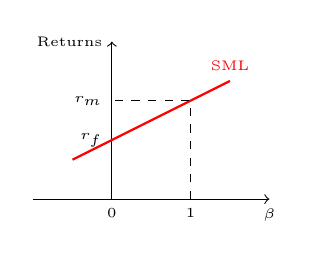
\begin{tikzpicture}
    % Draw axises
    \draw[->] (-1,0) -- (2,0) node[anchor=north] {\tiny $\beta$}; % X (beta) axis
    \draw[->] (0,0) -- (0,2) node[anchor=east] {\tiny Returns}; % Strike Price axis
    % Draw SML
    \draw[-,thick,red] (-0.5,0.5) -- (1.5,1.5) node[anchor=south] {\tiny SML};

    \draw[dashed] (1,0) -- (1,1.25) -- (0,1.25);

    % Label values
    \node[anchor=north] at (0,0) {\tiny $0$};
    \node[anchor=north] at (1,0) {\tiny $1$};
    \node[anchor=east] at (0,0.75) {\tiny $r_f$};
    \node[anchor=east] at (0,1.25) {\tiny $r_m$};
\end{tikzpicture}
\begin{itemize}
    \item Slope = market risk premium $(E[r_m] - r_f)$.
    \item An asset with a $\beta$ of 0 has an expected return = the risk-free rate $r_f$.
    \item An asset with a $\beta$ of 1 has an expected return = the market return $E[r_m]$.
\end{itemize}
\end{multicols}
\begin{tabular}{l|l}
    \textbf{CML} & \textbf{SML} \\
    \hline
    Plots $E[r]$ vs $\sigma$ & $E[r]$ vs asset $\beta$ \\
    \multicolumn{2}{l}{Passes thru risk-free asset \& tangency portfolio} \\
    Slope=Max Sharpe ratio & Mkt risk premium \\
    All indiv. risky assets lie below & lie on \\
    \hline
\end{tabular}

\subsection{Options}

\Red{Options}
Derivative contracts specifying \textbf{a right} to \textbf{buy (call option)} or \textbf{sell (put option)} an underlying asset at a specified price $K$ (the \textbf{strike/exercise price}) on or before a specified date $T$ (the \textbf{expiration/maturity date}).

\begin{itemize}
    \item \Blue{Call option}: right to buy the underlying asset at the strike price.
    \item \Blue{Put option}: right to sell the underlying asset at the strike price.
\end{itemize}

Exercise style:
\begin{itemize}
    \item \Blue{American option}: can be exercised at any time before expiration.
    \item \Blue{European option}: can only be exercised at expiration.
\end{itemize}

\subsubsection{Option Payoff curves}

\begin{itemize}
    \item \Blue{$S$} Price of the underlying asset at expiration
    \item \Blue{$K$} Strike price of option
    \item \Hint{Payoff $\neq$ Profit}. To get profit (net payoff), need to subtract the option's cost.
\end{itemize}

\begin{multicols}{2}
\tiny \textbf{Payoff of buying a Call}
$\max(0, S - K)$
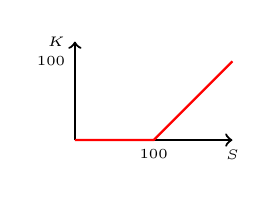
\begin{tikzpicture}
    % Draw lines
    \draw[->,thick] (0,0) -- (2,0) node[anchor=north] {\tiny $S$}; % Asset Price axis
    \draw[->,thick] (0,0) -- (0,1.25) node[anchor=east] {\tiny $K$}; % Strike Price axis
    % Draw payoff lines
    \draw[-,thick,red] (0,0) -- (1,0) -- (2,1);

    % Label values
    \node[anchor=north] at (1,0) {\tiny $100$};
    \node[anchor=east] at (0,1) {\tiny $100$};
\end{tikzpicture}

\tiny \textbf{Payoff of buying a Put}
$\max(0, K - S)$
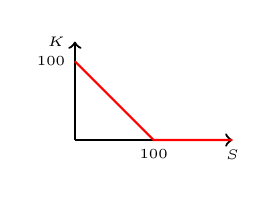
\begin{tikzpicture}
    % Draw lines
    \draw[->,thick] (0,0) -- (2,0) node[anchor=north] {\tiny $S$}; % Asset Price axis
    \draw[->,thick] (0,0) -- (0,1.25) node[anchor=east] {\tiny $K$}; % Strike Price axis
    % Draw payoff lines
    \draw[-,thick,red] (0,1) -- (1,0) -- (2,0);

    % Label values
    \node[anchor=north] at (1,0) {\tiny $100$};
    \node[anchor=east] at (0,1) {\tiny $100$};
\end{tikzpicture}

\tiny \textbf{Payoff of selling a Call}
$-\max(0, S - K)$
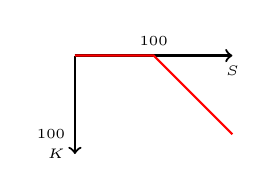
\begin{tikzpicture}
    % Draw lines
    \draw[->,thick] (0,0) -- (2,0) node[anchor=north] {\tiny $S$}; % Asset Price axis
    \draw[->,thick] (0,0) -- (0,-1.25) node[anchor=east] {\tiny $K$}; % Strike Price axis
    % Draw payoff lines
    \draw[-,thick,red] (0,0) -- (1,0) -- (2,-1);

    % Label values
    \node[anchor=south] at (1,0) {\tiny $100$};
    \node[anchor=east] at (0,-1) {\tiny $100$};
\end{tikzpicture}

\tiny \textbf{Payoff of selling a Put}
$-\max(0, K - S)$
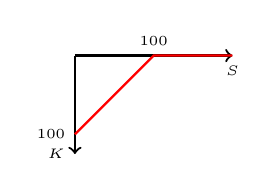
\begin{tikzpicture}
    % Draw lines
    \draw[->,thick] (0,0) -- (2,0) node[anchor=north] {\tiny $S$}; % Asset Price axis
    \draw[->,thick] (0,0) -- (0,-1.25) node[anchor=east] {\tiny $K$}; % Strike Price axis
    % Draw payoff lines
    \draw[-,thick,red] (0,-1) -- (1,0) -- (2,0);

    % Label values
    \node[anchor=south] at (1,0) {\tiny $100$};
    \node[anchor=east] at (0,-1) {\tiny $100$};
\end{tikzpicture}
\end{multicols}

Payoff curves of other assets that can be used with options:
\begin{multicols}{2}
\tiny Payoff of underlying asset
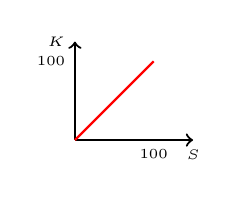
\begin{tikzpicture}
    % Draw lines
    \draw[->,thick] (0,0) -- (1.5,0) node[anchor=north] {\tiny $S$}; % Asset Price axis
    \draw[->,thick] (0,0) -- (0,1.25) node[anchor=east] {\tiny $K$}; % Strike Price axis
    % Draw payoff lines
    \draw[-,thick,red] (0,0) -- (1,1);

    % Label values
    \node[anchor=north] at (1,0) {\tiny $100$};
    \node[anchor=east] at (0,1) {\tiny $100$};
\end{tikzpicture}

\tiny Payoff of a \$100 FV ZC Bond
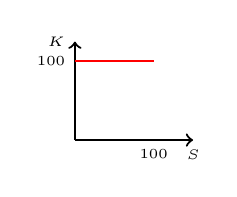
\begin{tikzpicture}
    % Draw lines
    \draw[->,thick] (0,0) -- (1.5,0) node[anchor=north] {\tiny $S$}; % Asset Price axis
    \draw[->,thick] (0,0) -- (0,1.25) node[anchor=east] {\tiny $K$}; % Strike Price axis
    % Draw payoff lines
    \draw[-,thick,red] (0,1) -- (1,1);

    % Label values
    \node[anchor=north] at (1,0) {\tiny $100$};
    \node[anchor=east] at (0,1) {\tiny $100$};
\end{tikzpicture}
\end{multicols}

\subsubsection{Option payoff and profit}

\begin{itemize}
    \item \Blue{$r$} Risk-free interest rate (EAR)
    \item \Blue{$C$} Call option price
    \item \Blue{$P$} Put option price
\end{itemize}

\Blue{Call option}
\begin{tabular}{c|c|c|c}
    & $S < K$ & $S = K$ & $S > K$ \\
    \hline
    Payoff & $0$ & $0$ & $S - K$ \\
    Profit & $-C (1+r)^T$ & $-C (1+r)^T$ & $S - K - C (1+r)^T$ \\
\end{tabular}

\Blue{Put option}
\begin{tabular}{c|c|c|c}
    & $S < K$ & $S = K$ & $S > K$ \\
    \hline
    Payoff & $K - S$ & $0$ & $0$ \\
    Profit & $K - S - P(1+r)^T$ & $- P(1+r)^T$ & $- P(1+r)^T$ \\
\end{tabular}

An option is
\begin{itemize}
    \item \Blue{in-the-money} if it has positive payoff at expiration. A call option is in-the-money if $S > K$, and a put option is in-the-money if $S < K$.
    \item \Blue{out-of-the-money} if it has zero payoff at expiration. A call option is out-of-the-money if $S < K$, and a put option is out-of-the-money if $S > K$.
    \item \Blue{at-the-money} if it has zero payoff at expiration. A call option is at-the-money if $S = K$, and a put option is at-the-money if $S = K$.
\end{itemize}

\Red{Put-call parity} following portfolios have the same payoff at expiration:
\begin{enumerate}
    \item \Blue{Long call with strike price $K$ + Bond with face value $K$}

    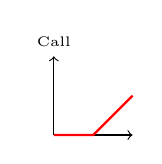
\begin{tikzpicture}
        % Draw lines
        \draw[->] (0,0) -- (1,0); % Asset Price axis
        \draw[->] (0,0) -- (0,1) node[anchor=south] {\tiny Call}; % Strike Price axis
        % Draw payoff lines
        \draw[-,thick,red] (0,0) -- (0.5,0) -- (1,0.5);
    \end{tikzpicture}
    \raisebox{4ex}{+}
    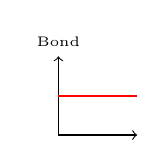
\begin{tikzpicture}
        % Draw lines
        \draw[->] (0,0) -- (1,0); % Asset Price axis
        \draw[->] (0,0) -- (0,1) node[anchor=south] {\tiny Bond}; % Strike Price axis
        % Draw payoff lines
        \draw[-,thick,red] (0,0.5) -- (1,0.5);
    \end{tikzpicture}
    \raisebox{4ex}{=}
    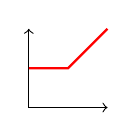
\begin{tikzpicture}
        % Draw lines
        \draw[->] (0,0) -- (1,0); % Asset Price axis
        \draw[->] (0,0) -- (0,1); % Strike Price axis
        % Draw payoff lines
        \draw[-,thick,red] (0,0.5) -- (0.5,0.5) -- (1,1);
    \end{tikzpicture}
    \item \Blue{Long put with strike price $K$ + Underlying asset}

    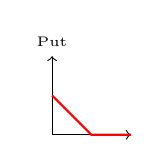
\begin{tikzpicture}
        % Draw lines
        \draw[->] (0,0) -- (1,0); % Asset Price axis
        \draw[->] (0,0) -- (0,1) node[anchor=south] {\tiny Put}; % Strike Price axis
        % Draw payoff lines
        \draw[-,thick,red] (0,0.5) -- (0.5,0) -- (1,0);
    \end{tikzpicture}
    \raisebox{4ex}{+}
    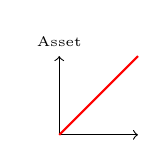
\begin{tikzpicture}
        % Draw lines
        \draw[->] (0,0) -- (1,0); % Asset Price axis
        \draw[->] (0,0) -- (0,1) node[anchor=south] {\tiny Asset}; % Strike Price axis
        % Draw payoff lines
        \draw[-,thick,red] (0,0) -- (1,1);
    \end{tikzpicture}
    \raisebox{4ex}{=}
    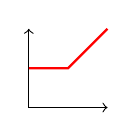
\begin{tikzpicture}
        % Draw lines
        \draw[->] (0,0) -- (1,0); % Asset Price axis
        \draw[->] (0,0) -- (0,1); % Strike Price axis
        % Draw payoff lines
        \draw[-,thick,red] (0,0.5) -- (0.5,0.5) -- (1,1);
    \end{tikzpicture}
\end{enumerate}

Given their identical payoffs, under no-arbitrage, they should have the same price:
\begin{itemize}
    \item $P_{call} + P_{bond} = P_{put} + P_{asset}$
    \item $C + K(1+r)^{-T} = P + S$
\end{itemize}

\Red{Binomial option pricing model} Iterative approach to price options that makes the following simplifications:
\begin{itemize}
    \item Discrete periods, in which stock price can either go up or down.
    \item We find the option price by a \textit{no arbitrage} argument. Price is equal to the cost of purchasing a \textit{replicating portfolio} whose payoffs match the option payoff in each state. \Eg, for a call, we solve: $\begin{cases}
        a S_u + b B_u &= C_u \\
        a S_d + b B_d &= C_d
    \end{cases}$ where $a$ is the number of shares of stock, $b$ is the number of bonds, $S_u$ and $S_d$ are the stock prices if it goes up or down, and $C_u$ and $C_d$ are the call option prices if stock goes up or down.
    \item  Under the binomial assumptions, \Hint{the probability of a stock moves up or down is irrelevant}, and the price of options can be determined solely using: \begin{itemize}
        \item Current stock price $S_0$, interest rate $r$, strike price $K$ and time to maturity $T$;
        \item Magnitude of possible future changes of stock price (volatility), captured implicitly by the possible values the stock can take $S_u$ and $S_d$.
    \end{itemize}
\end{itemize}

\Red{Black-Scholes formula} Taking the limit of binomial model as the number of periods gets large, we obtain the B-S formula for the price of a European call option without dividends:
\fbox{$C(S, K, T, r, \sigma) = S \cdot N(x) - K(1 + r)^{-T} \cdot N(x - \sigma \sqrt{T})$}
\begin{itemize}
    \item \Blue{$S$} current value of the underlying asset (in \$)
    \item \Blue{$K$} strike price of the option (in \$)
    \item \Blue{$T$} option maturity (in years)
    \item \Blue{$r$} annual risk-free interest rate
    \item \Blue{$\sigma$} annualized standard deviation of the underlying asset's return (volatility)
    \item \Blue{$N(\cdot)$} cumulative normal distribution function (\texttt{NORM.S.DIST(x, TRUE)}). These $N(\cdot)$ terms \Hint{capture the replicating portfolio weights}.
    \item \Blue{$x$} \fbox{$x = \frac{\ln\left(\frac{S}{K(1+r)^{-T}}\right)}{\sigma \sqrt{T}} + \frac{1}{2} \sigma \sqrt{T}$}
\end{itemize}

\Green{\Eg \underline{True} statement} \textit{According to the Black-Scholes model, holding all else equal, an increase in the expected idiosyncratic volatility of Apple's stock return will increase the value of a call option on Apple stock.} \Hint{The B\&S formula considers the volatility of the underlying
asset's price, which includes idiosyncratic volatility. The value of a call option increases with volatility because it increases the possible upside for the option holder without affecting the downside, which is limited by design.}

\Green{\Eg Harvesting and selling a large volume of wheat in three months' time.} Worries about market price $S_t$ may drop further between now and harvest. Consider 2 possible derivatives strategies to hedge against this risk. Underlying asset is 1 bushel of wheat. Expiration date $T$ is in 3 months.
\begin{enumerate}
    \item \Green{First possibility is to take a short position in (\ie sell) a forward contract, with a forward price $F = \$6$ per bushel.} Draw a diagram of wheat revenue per bushel (Y) vs market price of wheat $S_t$ (X) after buying this contract. \begin{multicols}{2}
        \Hint{The forward contract locks in the price of wheat at $F = \$6$ per bushel, so this is your date-$T$ revenue per bushel regardless of the future price of wheat.}
        \begin{tikzpicture}
            % Draw lines
            \draw[->,thick] (0,0) -- (1.5,0) node[anchor=north] {\tiny $S_T$};
            \draw[->,thick] (0,0) -- (0,1.5) node[anchor=south] {\tiny Rev}; % Strike Price axis
            % Draw payoff lines
            \draw[-,thick,red] (0,0.5) -- (1.5,0.5);
            % Label values
            \node[anchor=east] at (0,0.5) {\tiny $F = 6$};
        \end{tikzpicture}
    \end{multicols}
    \item \Green{Second possibility is to buy a European put option with a strike price $K = \$6$ per bushel.} Draw a diagram of wheat revenue per bushel (Y) vs market price of wheat $S_t$ (X) after buying this contract. \begin{multicols}{2}
        \Hint{The put opt gives you the right to sell wheat at $K = \$6$, so this is the min rev in 3mo. If price above $K$, will sell on the spot market and receive rev equal to the market price $S_T$.}
        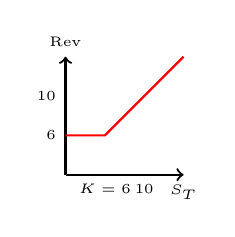
\begin{tikzpicture}
            % Draw lines
            \draw[->,thick] (0,0) -- (1.5,0) node[anchor=north] {\tiny $S_T$};
            \draw[->,thick] (0,0) -- (0,1.5) node[anchor=south] {\tiny Rev}; % Strike Price axis
            % Draw payoff lines
            \draw[-,thick,red] (0,0.5) -- (0.5,0.5) -- (1.5,1.5);
            % Label values
            \node[anchor=north] at (0.5,0) {\tiny $K = 6$};
            \node[anchor=east] at (0,0.5) {\tiny $6$};
            \node[anchor=east] at (0,1) {\tiny $10$};
            \node[anchor=north] at (1,0) {\tiny $10$};
        \end{tikzpicture}
    \end{multicols}
    \item \Green{Consioder the \underline{net} payoff (rev - hedging costs) under the 2 possible strategies}. If the price of wheat in 3mo is $S_T = \$3$ per bushel, which of the two strategies will provide a higher net payoff?
    \Hint{The forward contract yields a higher net payoff as it has no upfront premium, unlike the put option. The put's premium, paid for potential upside if prices exceed \$6, results in a lower net payoff if prices remain below \$6 and this upside is not realized.}
\end{enumerate}

\subsubsection{Real options}
Option-like payoffs appear in many contexts outside of financial markets. Management can be thought of as the act of creating and optimally exercising real options. \Green{\Eg} follow-on products, R\&D  investments, delaying product launches, abandoning projects, etc.

\end{multicols}
\end{document}